\documentclass[sigconf]{acmart}

\usepackage{bm}
\usepackage{mathrsfs}
\usepackage{enumerate}
\usepackage{setspace}

\usepackage[lined,boxed,ruled,vlined]{algorithm2e}
\SetKwInOut{Input}{Input}
\SetKwInOut{Output}{Output}

\author{Seung Gyu Hyun}
\affiliation{%
  \institution{Cheriton School of Computer Science}
  \institution{University of Waterloo}
}
\email{sghyun@edu.uwaterloo.ca}

\author{Romain Lebreton}
\affiliation{
  \institution{LIRMM}
  \institution{Universit\'e de Montpellier}
}
\email{romain.lebreton@lirmm.fr}

\author{\'Eric Schost}
\affiliation{%
  \institution{Cheriton School of Computer Science}
  \institution{University of Waterloo}
}
\email{eschost@uwaterloo.ca}

\newcommand{\va}{\ensuremath{\mathsf{a}}}
\newcommand{\vb}{\ensuremath{\mathsf{b}}}
\newcommand{\vc}{\ensuremath{\mathsf{c}}}
\newcommand{\ve}{\ensuremath{\mathsf{e}}}
\newcommand{\vf}{\ensuremath{\mathsf{f}}}
\newcommand{\vg}{\ensuremath{\mathsf{g}}}
\newcommand{\vh}{\ensuremath{\mathsf{h}}}
\newcommand{\vi}{\ensuremath{\mathsf{i}}}
\newcommand{\vr}{\ensuremath{\mathsf{r}}}
\newcommand{\vu}{\ensuremath{\mathsf{u}}}
\newcommand{\vv}{\ensuremath{\mathsf{v}}}
\newcommand{\vx}{\ensuremath{\mathsf{x}}}
\newcommand{\vy}{\ensuremath{\mathsf{y}}}

\newcommand{\mA}{\ensuremath{\mathsf{A}}}
\newcommand{\mB}{\ensuremath{\mathsf{B}}}
\newcommand{\mC}{\ensuremath{\mathsf{C}}}
\newcommand{\mD}{\ensuremath{\mathsf{D}}}
\newcommand{\mG}{\ensuremath{\mathsf{G}}}
\newcommand{\mH}{\ensuremath{\mathsf{H}}}
\newcommand{\mI}{\ensuremath{\mathsf{I}}}
\newcommand{\mJ}{\ensuremath{\mathsf{J}}}
\newcommand{\mM}{\ensuremath{\mathsf{M}}}
\newcommand{\mN}{\ensuremath{\mathsf{N}}}
\newcommand{\mP}{\ensuremath{\mathsf{P}}}
\newcommand{\mR}{\ensuremath{\mathsf{R}}}
\newcommand{\mS}{\ensuremath{\mathsf{S}}}
\newcommand{\mT}{\ensuremath{\mathsf{T}}}
\newcommand{\mV}{\ensuremath{\mathsf{V}}}
\newcommand{\mW}{\ensuremath{\mathsf{W}}}
\newcommand{\mX}{\ensuremath{\mathsf{X}}}
\newcommand{\mY}{\ensuremath{\mathsf{Y}}}
\newcommand{\mZ}{\ensuremath{\mathsf{Z}}}

\newcommand{\K}{\ensuremath{\mathbb{K}}}
\newcommand{\Q}{\ensuremath{\mathbb{Q}}}
\newcommand{\Z}{\ensuremath{\mathbb{Z}}}

\newcommand{\M}{\ensuremath{\mathscr{M}}}
\newcommand{\I}{\ensuremath{\mathscr{I}}}
\newcommand{\CA}{\ensuremath{\mathscr{C}_\mA}}
\renewcommand{\P}{\ensuremath{\mathscr{P}}}

\newcommand{\mx}{\ensuremath{\nu}}
\newcommand{\mn}{\ensuremath{\mu}}

\newcommand{\lm}{\ensuremath{\operatorname{lm}}}
\newcommand{\rank}{\ensuremath{\operatorname{rank}}}
\newcommand{\DACp}{\ensuremath{\mathsf{DAC}}}
\newcommand{\DACQ}{\ensuremath{\mathsf{DAC}_\Q}}
\newcommand{\Iter}{\ensuremath{\mathsf{Iter}}}
\newcommand{\Raise}{\textbf{raise} error}


\DeclareBoldMathCommand{\bF}{F}
\DeclareBoldMathCommand{\bh}{h}
\DeclareBoldMathCommand{\bu}{u}
\DeclareBoldMathCommand{\bx}{x}
\DeclareBoldMathCommand{\by}{y}

\newcommand{\Otilde}[1]{\ensuremath{O\tilde{~}(#1)}} % soft O for complexity
\newcommand{\todo}[1]{(\textbf{todo:} #1)} 
\newcommand{\why}{\textbf{why?}} 

\newtheorem{pbm}{Problem}
\renewcommand{\thepbm}{\Alph{pbm}} % "letter-numbered" theorems
% \newtheorem{definition}{Definition}
% \newtheorem{theorem}[definition]{Theorem}
% \newtheorem{corollary}[definition]{Corollary}
% \newtheorem{proposition}[definition]{Proposition}
% \newtheorem{lemma}[definition]{Lemma}

\theoremstyle{acmdefinition}
\newtheorem{remark}[theorem]{Remark}
% \newtheorem{algo}{Algorithm}

\def\gathen#1{{#1}}

\acmConference[ISSAC]{International Symposium on Symbolic and Algebraic Computation}{2017}{Kaiserslautern, Germany}
\acmYear{2017}
\copyrightyear{2017}
\setcopyright{rightsretained}


\title{Algorithms for structured linear systems solving and their
  implementation}


\begin{abstract}
  There exists a vast literature dedicated to algorithms for
  structured matrices, but relatively few descriptions of actual
  implementations and their practical performance. In this paper, we
  consider the problem of solving Cauchy-like systems, and its
  application to mosaic Toeplitz systems, in two contexts: first in
  the unit cost model (which is a good model for computations over
  finite fields), then over $\Q$. We introduce new variants of
  previous algorithms and describe an implementation of these
  techniques and its practical behavior. We pay a special attention to
  particular cases such as the computation of algebraic approximants.
\end{abstract}

\begin{document}


\maketitle

%%%%%%%%%%%%%%%%%%%%%%%%%%%%%%%%%%%%%%%%%%%%%%%%%%%%%%%%%%%%
%%%%%%%%%%%%%%%%%%%%%%%%%%%%%%%%%%%%%%%%%%%%%%%%%%%%%%%%%%%%
%%%%%%%%%%%%%%%%%%%%%%%%%%%%%%%%%%%%%%%%%%%%%%%%%%%%%%%%%%%%

\vspace{-5px}
\section{Introduction}

In this paper, we discuss linear algebra algorithms inspired by the
following kind of question: given polynomials such as
\[
\left\{
\begin{array}{rcl}
t_0 &=& 8x^4 - 8x^2 + 1\\
t_1 &=& 16x^5 - 20x^3 + 5x\\
t_2 &=& 32x^6 - 48x^4 + 18x^2 - 1,
\end{array}
\right.
\]
find that the relation $t_0-2x t_1+t_2=0$ holds (this is the
recurrence between Chebyshev polynomials of the first kind).  

More precisely, given input polynomials $(t_0,\dots,t_{s-1})$ over a
field $\K$, together with integers $(n_0,\dots,n_{s-1})$ and $\sigma$,
the {\em Hermite-Pad\'e} approximation problem asks to compute
polynomials $(p_0,\dots,p_{s-1})$, not all zero, such that $\deg(p_i)
< n_i$ holds for all $i$, and such that we have $p_0 t_0 + \cdots +
p_{s-1} t_{s-1}=O(x^\sigma)$. There exist numerous applications to
this type of question, very important particular cases being {\em
  algebraic approximants} (with $t_i =f^i$, for some given $f$) or
{\em differential approximants} (with $t_i =d^if/dx^i$, for some given
$f$); see for instance~\cite[Chapitre~7]{BoChGiLeLeSaSc17}.

Expressed in the canonical monomial bases, the matrix of a
Hermite-Pad\'e problem has size $\sigma \times (n_0 + \cdots +
n_{s-1})$, and consists of $s$ lower triangular Toeplitz blocks. More
generally, our goal in this paper is to compute efficiently elements
in the kernel of {\em mosaic Toeplitz} matrices~\cite{HeAm88}, that
is, $m \times n$ matrices $\mT=(\mT_{i,j})_{1 \le i \le p,1 \le j \le
  q}$ with a $p \times q$ block structure, each of the $pq$ blocks
$\mT_{i,j}$ being Toeplitz.

An $m \times n$ Toeplitz matrix
$\mT=(t_{i-j})_{1\le i \le m, 1 \le j \le n}$ can be succinctly
represented by the polynomial
$P_\mT=t_{-n+1} + t_{-n+2} x + \cdots + t_{m-1} x^{m+n-2}$;
multiplication of $\mT$ by a vector $\vb=[b_0~\cdots~b_{n-1}]^t$
amounts to computing $P_\mT P_\vb \bmod x^{m+n-1}$ and keeping the
coefficients of degrees $n-1,\dots,m+n-2$.  More generally, a mosaic
Toeplitz $\mT=(\mT_{i,j})_{1 \le i \le p,1 \le j \le q}$ can be
described by a sequence of $pq$  polynomials
$\P=(P_{\mT_{i,j}})_{1 \le i \le p,1 \le j \le q}$, together
with the sequences $I=(m_1,\dots,m_p)$ and $J=(n_1,\dots,n_q)$ giving
the row-sizes and column-sizes of the blocks. Then, our main
problem is as follows.
%
\vspace{-5px}
\begin{pbm}\label{pb:mosaic}
  Given $\P$ and integers $I,J$ as above, 
  defining a mosaic Toeplitz matrix $\mT$, find a non-zero
  vector in the kernel of $\mT$.
\end{pbm}
\vspace{-5px}
%
We consider two situations, first over an arbitrary field $\K$,
counting all operations in $\K$ at unit cost, then over $\Q$, taking
bit-size into account. In all this paper, we closely follow the
existing formalism of {\em structured matrix computations} developed
in previous work by Morf~\cite{Morf80},
Bitmead-Anderson~\cite{BiAn80}, Kailath and
co-authors~\cite{KaKuMo79,KaSa99}, Pan~\cite{Pan90,Pan92},
Kaltofen~\cite{Kaltofen94}, Cardinal~\cite{Cardinal99}, etc.

We complement the existing literature as follows. First, we define a
class of Cauchy-like matrices (see definitions below) for which
the matrix-vector product is faster by a constant factor than previous
designs. Next, we show how Pan's technique of ``multiplicative
transformation'' of operators results in matrices that have generic
rank profile (with high probability), so that further regularization
is not needed in general. We then describe an improved iterative
algorithm (of quadratic complexity with respect to the matrix size),
that makes use of fast matrix multiplication; finally, for matrices
defined over $\Q$, we introduce a divide-and-conquer algorithm as an
alternative to Newton iteration, and we show how it can be improved in
the case of algebraic approximation.

Another contribution of this paper is a discussion of the design and
practical performance of a C++ implementation of these algorithms.  To
our knowledge, only a few papers address these methods from the
practical viewpoint. An early reference is~\cite{SeShSp82}, which
concludes that the divide-and-conquer (MBA) algorithm for solving
Toeplitz matrices in quasi-linear time would require matrices of size
$10^6$ to break even with quadratic-time algorithms; a more recent
article~\cite{Huckle94} estimates the crossover point to be around
$8000$. 

Our experiments first consider computations over finite fields.  We
assess the practical impact of fast matrix multiplication for
structured matrix algorithms (such as in the new algorithm mentioned
above, or those in~\cite{BoJeSc08,BoJeMoSc16}), and we estimate for
what matrix size quasi-linear algorithms become effective (with much
lower crossover points than above). In the context of computations
over $\Q$, we show that our divide-and-conquer algorithm outperforms
Newton iteration consistently, and we demonstrate significant
speed-ups for the case of algebraic approximants.

We start in Section~\ref{sec:basics} with a review of basic results on
structured matrices, including a discussion of transformation of
operators and regularization. Section~\ref{sec:abstract} describes
algorithms applicable in a unit cost model, with in particular a new
algorithm that uses fast matrix multiplication, and a discussion of
the practical performance of these algorithms. Finally,
Section~\ref{sec:lifting} presents lifting algorithms for structured
matrices, and the corresponding implementation.

%%%%%%%%%%%%%%%%%%%%%%%%%%%%%%%%%%%%%%%%%%%%%%%%%%%%%%%%%%%%
%%%%%%%%%%%%%%%%%%%%%%%%%%%%%%%%%%%%%%%%%%%%%%%%%%%%%%%%%%%%
%%%%%%%%%%%%%%%%%%%%%%%%%%%%%%%%%%%%%%%%%%%%%%%%%%%%%%%%%%%%

\vspace{-5px}
\section{Basic results}\label{sec:basics}

This section reviews background material on structured matrices; for a
more comprehensive treatment, we refer the reader to~\cite{Pan01}.


\smallskip\noindent{\bf \small Overview.}  Developed
in~\cite{KaKuMo79}, the {\it displacement operator} approach
associates to a matrix $\mA$ its displacement $\nabla(\mA)$, that is, the
image of $\mA$ under a \textit{displacement operator}~$\nabla$.  Then,
we say that $\mA$ is structured with respect to $\nabla$ if $\nabla(\mA)$
has a small rank compared to its size; the rank of $\nabla(\mA)$ is
called the \textit{displacement rank} of $\mA$ with respect to
$\nabla$. A prominent example is the family of so-called {\em
  Toeplitz-like} matrices, which are structured for the Toeplitz
displacement operator
% \vspace{-1px}
\begin{eqnarray*}
  \phi: \mA & \mapsto & \left( \mZ_m \mA - \mA \mZ_n \right) = 
                        (\mA \downarrow) - (\mA \leftarrow)
\end{eqnarray*}
%\vspace{-1px}
where the $n \times n$ lower shift matrix $\mZ_n$ is the matrix
with ones below the diagonal.  The displacement rank of a Toeplitz
matrix for this operator is at most two; the displacement rank of a
mosaic Toeplitz with a $p \times q$ block structure is at most $p+q$.

The key idea of most algorithms for structured matrices is summarized
by Pan's motto~\cite{Pan01}: compress, operate, decompress. Indeed,
for $\mA$ of size $m \times n$ over a field $\K$, if $\nabla(\mA)$ has
rank~$\alpha$, it can be represented using few elements through {\it
  $\nabla$-generators}, that is, two matrices $(\mG,\mH)$ in
$\K^{m\times \alpha} \times \K^{n\times \alpha}$, with $\nabla(\mA) =
\mG \mH^t$; $\alpha$ is the {\em length} of the generators. The main
idea behind algorithms for structured matrices is to use generators as
a compact data structure, involving $\alpha (m+n)$ field elements
instead of $mn$.

\smallskip\noindent{\bf \small Cauchy-like matrices.}  Beyond the
Toeplitz structure (and the directly related Hankel one), two other
important cases are the so-called Vandermonde and Cauchy
structures. While the case of Toeplitz-like matrices was the first one
to be studied in detail, we will actually focus on Cauchy-like
matrices, as we will see that this particular structure is quite
convenient to work with.

For a sequence $\vu=(u_1,\dots,u_m)$ in $\K^m$, let $\mD_\vu \in
\K^{m\times m}$ be the diagonal matrix with entries
$u_1,\dots,u_m$. Then, given $\vu$ as above and $\vv$ in $\K^n$, we will
consider the operator $\nabla_{\vu,\vv}: \mA \in \K^{m\times n} \mapsto \mD_\vu
\mA - \mA \mD_\vv$; {\em Cauchy-like} matrices (with respect to the
choice of $\vu$ and $\vv$) are those matrices $\mA$ for which
$\nabla_{\vu,\vv}(\mA)$ has small rank.

Let $\vu,\vv$ be given and suppose that $u_i \ne v_j$ holds for all
$i,j$. Then, the operator $\nabla_{\vu,\vv}$ is invertible: given
$\nabla_{\vu,\vv}$-generators $(\mG,\mH)$ of length $\alpha$ for $\mA$, we can reconstruct $\mA$ as
\begin{equation}\label{eq:recA}
\mA = \sum_{i=1}^\alpha
\mD_{\vg_i} 
\mC_{\vu,\vv}\,\mD_{\vh_i},\ \ \ 
\mC_{\vu,\vv}=\begin{bmatrix}
\frac 1{u_i-v_j}
\end{bmatrix}_{\substack{1 \leq i \leq m\\1 \leq j \leq n}},
\end{equation}
where $\vg_i$ and $\vh_i$ are the $i$th columns of respectively $\mG$
and~$\mH$, and  matrix $\mC_{\vu,\vv}$ is known as a {\em Cauchy
  matrix}. Remark that we can
equivalently rewrite $\mA$ as
\begin{equation}\label{eq:recA2}
\mA= (\mG \mH^t) \odot \mC_{\vu,\vv},
\end{equation}
where $\odot$ denotes the entrywise product.

We will have to handle submatrices of $\mA$ through their
generators. The fact that $\mD_{\vu}$ and $\mD_{\vv}$ are diagonal
matrices makes this easy (this is one of the aspects in which the
Cauchy structure behaves more simply than the Toeplitz one).  Suppose
that $(\mG,\mH)$ are generators for $\mA$, with respect to the
operator $\nabla_{\vu,\vv}$, and let $\vu_I=(u_i)_{i \in I}$ and
$\vv_J=(v_j)_{j \in J}$ be subsequences of respectively $\vu$ and
$\vv$, corresponding to entries of indices $I$ and $J$. Let
$\mA_{I,J}$ be the submatrix of $\mA$ obtained by keeping rows and
columns of indices respectively in $I$ and $J$, and let
$(\mG_I,\mH_J)$ be the matrices obtained from $(\mG,\mH)$ by
respectively keeping rows of $\mG$ of indices in $I$, and rows of
$\mH$ of indices in $J$. Then, $(\mG_I,\mH_J)$ is a
$\nabla_{\vu_I,\vv_J}$-generator for $\mA_{I,J}$.

Another useful property relates to inverses of Cauchy-like matrices.
If a matrix $\mA \in \K^{n\times n}$ is invertible, and is structured
with respect to an operator $\nabla_{\vu,\vv}$, its inverse is
structured with respect to $\nabla_{\vv,\vu}$: if $\mD_\vu \mA - \mA
\mD_\vv = \mG \mH^t$, one easily deduces that $\mD_\vv \mA^{-1} -
\mA^{-1} \mD_\vu = - (\mA^{-1} \mG) (\mA^{-t} \mH)^t$, where $\mA^{-t}$
is a shorthand for $(\mA^{-1})^t$.


\smallskip\noindent{\bf \small Algorithms.}  In most of the paper, we
give costs in an algebraic model, counting base field operations at
unit cost (in Section~\ref{sec:lifting}, we work over $\Q$ and use 
a boolean model).

We let $\M$ be such that over any ring, polynomials of degree at most
$d$ can be multiplied in $\M(d)$ base ring operations; we also assume
that the super-linearity assumptions of~\cite[Chapter~8]{GaGe13}
hold. Using the Cantor-Kaltofen algorithm~\cite{CaKa91}, we can take
$\M(d)\in O(d \log(d)\log\log(d))$. We let $\omega$ be a feasible
exponent for linear algebra, in the sense that matrices of size $n$
can be multiplied in $O(n^\omega)$ base ring operations over any ring;
the best bound to date is $\omega < 2.38$~\cite{CoWi90, LeGall14}.  We
will have to compute rank and rank profile of dense matrices; the cost
reduces to that of matrix multiplication~\cite{IbMoHu82}. The notation
$\Otilde{\,}$ indicates that we omit polylogarithmic terms.

Matrix-vector multiplication with $\mC_{\vu,\vv}$ reduces to degree
$n$ polynomial interpolation at the points $\vv$ and evaluation at the
points $\vu$. Using fast polynomial evaluation and interpolation, this
can be done in time $O(\M(\mx)\log(\mx))$, with $\mx=\max(m,n)$; thus, we
can multiply matrix $\mA$ of~\eqref{eq:recA} by a vector in time
$O(\alpha \M(\mx)\log(\mx))\subset \Otilde{\alpha \mx}$.
In~\cite[Theorem~4.7.3]{Pan01}, Pan shows that if the entries of both
$\vu$ and $\vv$ are in {\em geometric progression}, one can reduce the
cost of the matrix-vector multiplication by $\mC_{\vu,\vv}$ to
$O(\M(\mx))$, since polynomial evaluation or interpolation at $n$
points in geometric progression can be done in time $O(\M(n))$~\cite{Bluestein70,BoSc05};
then, multiplication by $\mA$ as above takes time
$O(\alpha\M(\mx))$.

\vspace{-2mm}

\begin{remark}\label{rmk:factor3}
We propose here a refinement of this idea, that allows us to
save a constant factor in runtime: we require that $\vu$ and $\vv$ be
geometric progressions with {\em the same ratio} $\tau$. Then, the
Cauchy matrix $\mC_{\vu,\vv}$ has entries $1/(u_i -
v_j) = 1/(u_1 \tau^{i-1} - v_1 \tau^{j-1})$, so it can be factored as
\vspace{-3px}
$$
\mC_{\vu,\vv}=\mD_{\tau^{-1}}
\begin{bmatrix}
\frac{1}{u_1 - v_1 \tau^{j-i}}
\end{bmatrix}_{\substack{1 \leq i \leq m\\1 \leq j \leq n}},
$$

\vspace{-3px}
\noindent where $\mD_{\tau^{-1}}$ is diagonal with entries
$(1,\tau^{-1},\tau^{-2},\dots,\tau^{1-m})$, and where the right-hand matrix
is Toeplitz. In the reconstruction formula~\eqref{eq:recA}, the
diagonal matrix $\mD_{\tau^{-1}}$ commutes with all matrices $\mD_{\vg_i}$, so
we can take it out of the sum. Hence, we replaced $\alpha$ evaluations
/ interpolations at geometric progressions by $\alpha$ product by
Toeplitz matrices, each of which can be done in a single polynomial
multiplication. The cost for a matrix-vector product by $\mA$ remains
$O(\alpha \M(\mx))$, but the constant in the big-O is lower: for $m=n$,
using middle product techniques~\cite{HaQuZi04,BoLeSc03}, the
cost goes down from $3\alpha \M(\mx) +O(\alpha \mx)$ to $\alpha \M(\mx)
+O(\alpha \mx)$. 
\end{remark}

If one needs to multiply $\mA$ by {\em several} vectors,
further improvements are possible: we mention without giving details
an algorithm from~\cite{BoJeMoSc16}, that itself
follows~\cite{BoJeSc08}, and which makes it possible to multiply $\mA$
by $\alpha$ vectors in time $O(\alpha^{\omega-1} \M(\mx))$ instead of
$O(\alpha^2 \M(\mx))$, by reduction to a sequence of polynomial matrix
multiplications.

\smallskip\noindent{\bf \small Reduction from mosaic Toeplitz to Cauchy structure.}
Our primary interest lies in mosaic
Toep\-litz matrices. An important insight of Pan~\cite{Pan90} shows
that one can reduce questions about Toeplitz-like matrices to ones
about Cauchy-like matrices (and conversely, if one wishes to), for a
moderate cost overhead. In this paragraph, we give details on 
this transformation, following~\cite[Chapter~4.8]{Pan01}.

To a vector $\vu$ in $\K^m$, let us  associate the
corresponding Vandermonde matrices
$
\mV_\vu = \left[\begin{smallmatrix}
u_i^{j-1}
\end{smallmatrix}\right]_{1 \leq i,j \leq m},
\mW_\vu = \left[\begin{smallmatrix}
u_j^{m-i}
\end{smallmatrix}\right]_{1 \leq i,j \leq m}.
$
%
For $\vu$ as above, $\vv$ in $\K^n$ and $\mT$ in $\K^{m\times n}$, we
let $\mA = \mV_\vu\, \mT\, \mW_\vv$; we now prove that if $\mT$ is
Toeplitz-like, $\mA$ is Cauchy-like.

The $\nabla_{\vu,\vv}$-generators of $\mA$ depend on the
$\phi$-generators of $\mT$, so let us start with those. If
$\mT=(\mT_{i,j})_{1 \le i \le p,1 \le j \le q}$ is mosaic Toeplitz of
size $m \times n$, with $\mT_{i,j}$ of size $m_i \times n_j$, we
define the following.

For $1 \le i \le p$, let $\mT_{i,*}$ be the block matrix
$[\mT_{i,1}~\cdots~\mT_{i,q}]$.  Let $\eta_i$ be the first row of
$\mT_{i,*}$, shifted left once, let $\eta'_i$ be the last row of
$\mT_{i,*}$, and finally let $\vh_i=(\eta'_{i-1}-\eta_i)$ (for $i=1$,
$\eta'_0$ is the zero vector); this is a row-vector of size $n$. If
$\ve_{i,n}$ denotes the row-vector of dimension $n$ with only a one at
index $i$, we also let $\vg_{i}$ be the transpose of
$\ve_{m_1 + \cdots +m_{i-1}+1,m}$.  For $1 \le j \le q$, define
$\mT_{*,j}$ similarly to $\mT_{i,*}$; $\lambda_j$ and $\lambda'_j$ are
its first and last columns, with now a downward shift for
$\lambda'_j$; in addition, their entry of index $m_1 + \cdots + m_j$
are set to zero. We define $\vg_{p+j}=(\lambda'_{j}-\lambda_{j+1})$
($\lambda_{q+1}$ is set to zero) and let
$\vh_{p+j}=\ve_{n_1 + \cdots +n_j,n}$.  With these definitions, the
matrices $\mG=[ \vg_1, \dots, \vg_{p+q} ]$ and
$\mH=[\vh^t_1, \dots, \vh^t_{p+q}]$ are $\phi$-generators of $\mT$.

To obtain $\mA$, we conjugate $\mT$ by Vandermonde matrices, since $
\mD_{\vu} \mV_{\vu} - \mV_{\vu} \mZ_m$ and $ \mW_{\vv} \mD_{\vv} -
\mZ_n \mW_{\vv}$ have small rank; explicitly, they are equal to
respectively $(\vu^m)^t \, \ve_{m,m}$ and $(\ve_{1,n})^t \, \vv^n$,
where $\vu^m = [ u_1^m , \dots,  u_n^m ]$,
and similarly for $\vv^n$. As a
consequence, since $\phi(\mT)=\mG \mH^t$, we have
\begin{align}\label{eq:gentoetogencau}
  \nabla_{\vu, \vv} \left( \mA \right) 
  % & =  \mD_{\vu}  \mV_{\vu} \mT  \mW_{\vv} - \mV_{\vu}  \mT  \mW_{\vv}  \mD_{\vv} \nonumber \\
  & =  \mV_{\vu}\, \phi(\mT)\, \mW_{\vv} 
  %% \\
  %% &   &
  + (\vu^m)^t \, \ve_{m,m}  \mT  \mW_{\vv} 
        - \mV_{\vu}  \mT  (\ve_{1,n})^t \, \vv^n. 
\end{align}
This motivates the following definitions. For $1 \le i \le p$, let
$\vh'_i=\vh_i \mW_\vv$ and also let $\vg'_{i}$ be the column of
$\mV_\vu$ of index $m_1 + \cdots +m_{i-1}+1$. For $1 \le j \le q$,
define $\vg'_{p+j} = \mV_\vu \vg_{p+j}$ and also let $\vh'_{p+j}$ be
the row of index $n_1 + \cdots +n_j$ in $\mW_\vv$.  We define
$\vg_{p+q+1} = (\vu^m)^t$, and $\vh_{p+q+1}$ as the last row of
$\mT \mW_\vv$; we also define $\vg_{p+q+2}$ as the first column of
$-\mV_\vu \mT$, and $\vh_{p+q+2} = \vv^n$.

By Eq.~(\ref{eq:gentoetogencau}),
$\mG'= [ \vg'_1  \cdots  \vg'_{p+q+2}]$ and
$\mH' =[ {\vh'_1}^t  \cdots  {\vh'_{p+q+2}}^t]$ are
$\nabla_{\vu,\vv}$-generators of $\mA$ of length $p+q+2$ (whereas
$\mT$ has $\phi$-generators of length $p+q$). The bottleneck in the
computation of $\mG'$ and $\mH'$ are $p$ left-products by $\mW_\vv$
and $q$ products by $\mV_\vu$.  If all entries of $\vu$ and $\vv$ are
in geometric progression, it takes time $O(p \M(n) + q \M(m))$.

\smallskip\noindent{\bf \small Regularization.}  In our algorithms for
Cauchy-like matrices, we will assume that the input matrix has {\em
  generic rank profile}, that is, that its leading principal minors of
size up to its rank are invertible.  Regularization for structured
matrices was introduced for this purpose by
Kaltofen~\cite{Kaltofen94}, for the Toeplitz structure. In our Cauchy
context, one could apply to $\mA$ as defined above the regularization
procedure from~\cite[Section~5.6]{Pan01}, which consists in replacing
$\mA$ by $\mA' = \mD_\vx \mC_{\va,\vu} \mA \mC_{\vv,\vb}\mD_\vy$,
for some new vectors $\vx,\va \in \K^m$ and $\vy,\vb \in
\K^n$. Theorem~5.6.2 in~\cite{Pan01} shows that if $\va,\vu$ consist
of $2m$ distinct scalars, and $\vb,\vv$ consist of $2n$ distinct
scalars, then there exists a non-zero polynomial $\Delta$ in the
entries of $\vx$ and $\vy$, of degree at most $\mn=\min(m,n)$ in each
block of variables, such that the non-vanishing of $\Delta$ implies
that $\mA'$ has generic rank profile (that theorem is stated for
square matrices, but the result holds in the rectangular case as
well).  The downside of this construction is that it requires to
compute a pair of generators of length $p+q+4$ for $\mA'$, involving
the multiplication of $\mG'$ and $\mH'$ by $\mC_{\va,\vu}$ and
$\mC_{\vv,\vb}$.

\smallskip

We now prove a new property, involving only
$\mA = \mV_\vu\, \mT\, \mW_\vv$ as above. For the rest of this
paragraph, we assume that the entries of $\vu$ and $\vv$ are
indeterminates over $\K$, and we show that $\mA$ has generic rank
profile; this will imply the same property for a generic choice of
$\vu,\vv$ with entries in $\K$. This construction is clearly favorable
over the one above, since it involves no extra computation on $\mA$.
Following the proof of~\cite[Theorem~5.6.2]{Pan01}, we can use the
Cauchy-Binet formula to express the minors of $\mA$ in terms of those
of $\mV_\vu$, $\mT$ and $\mW_\vv$. Let $i \le {\rm rank}(\mT)$ and let
$I=\{1,\dots,i\}$. The determinant $\delta_i$ of the $i$th leading
principal minor of $\mA$ is the sum over all
$J=\{j_1,\dots,j_i\} \subset \{1,\dots,m\}$ and
$K=\{k_1,\dots,k_i\} \subset \{1,\dots,n\}$ of
$\alpha_{I,J}\, \beta_{J,K}\, \gamma_{K,I}$, where $\alpha_{I,J}$ is
the determinant of $(\mV_\vu)_{I,J}$, $\beta_{J,K}$ is the determinant
of $\mT_{J,K}$, and $\gamma_{K,I}$ is the determinant of
$(\mW_\vv)_{K,I}$.

Let $<$ be the monomial ordering on the variables $u_1,\dots,u_i$,
$v_1,\dots,v_i$ that first sorts monomials using the lexicographic order on
$u_1,\dots,u_i$ with $u_1 < \dots < u_i$, and then breaks the ties using the
lexicographic order on $v_1,\dots,v_i$ with $v_1 > \dots > v_i$. If
$J=\{j_1,\dots,j_i\}$ with $j_1 < \dots < j_i$ then the leading monomial
(denoted $\lm(\cdot)$) of $\alpha_{I,J}$ is
$\vu^J := u_1^{j_1-1} \cdots u_i^{j_i-1}$.  Similarly if $K=\{k_1,\dots,k_i\}$
with $k_1 < \cdots < k_i$, then
$\vv^K := v_1^{n-k_1} \cdots v_i^{n-k_i}=\lm(\gamma_{K,I})$. Since $\mT$ is of
rank greater or equal to $i$, at least one of its $i$th minor $\beta_{J,K}$ does
not vanish. Let $J_{\max},K_{\max}$ be the pair of subsets that maximizes
$\vu^J \vv^K$ among those for which $\beta_{J,K} \neq 0$. Then we must have
$\lm(\det(\mA_{I,I})) = \vu^{J_{\max}} \vv^{K_{\max}}$, which shows that
$\det(\mA_{I,I})$ is non-zero. The partial degree of $\det(\mA_{I,I})$ in any variable
 is at most $\max(n,m)$. 

%% \todo{See if we can derive anything for geometric sequences $\vu, \vv$
%%   with the same ratio}

%%%%%%%%%%%%%%%%%%%%%%%%%%%%%%%%%%%%%%%%%%%%%%%%%%%%%%%%%%%%
%%%%%%%%%%%%%%%%%%%%%%%%%%%%%%%%%%%%%%%%%%%%%%%%%%%%%%%%%%%%
%%%%%%%%%%%%%%%%%%%%%%%%%%%%%%%%%%%%%%%%%%%%%%%%%%%%%%%%%%%%

\vspace{-5px}
\section{Over an abstract field}\label{sec:abstract}

In this section, we work over a field $\K$, and we explain how to
solve Problem~\ref{pb:mosaic} by using Pan's reduction to the
Cauchy-like Problem~\ref{pb:cauchy} below. Even though our goal is to
solve a linear system, the algorithms do slightly more: they compute
the inverse of a given matrix (or of a maximal minor thereof); this is
similar to what happens for dense matrices, where it is not known how
to solve linear systems with an exponent better than $\omega$.
Then, the main question of this section is the following (the
assumptions on the vectors $\vu,\vv$ are slightly stronger than the
one required for $\nabla_{\vu,\vv}$ to be invertible). 
%
% \vspace{-5px}
\begin{pbm}\label{pb:cauchy}
  Consider $\vu=(u_1,\dots,u_m)$ and $\vv=(v_1,\dots,v_n)$,
  such that $(\vu,\vv)$ has $m+n$ distinct entries. Given
  $\nabla_{\vu,\vv}$-generators of length $\alpha$ for $\mA$
  in $\K^{m \times n}$, with $\alpha \le \min(m,n)$, do the following.

  If $\mA$ does not have generic rank profile, raise an error;
  else, return $\nabla_{\vv',\vu'}$-generators for the inverse
    of the leading principal minor $\mA_r$ of $\mA$ of order $r$, with
    $\vv'=(v_1,\dots,v_r)$, $\vu'=(u_1,\dots,u_r)$ and
    $r={\rm rank}(\mA)$.
\end{pbm}
% \vspace{-5px}
%
To solve an instance of Problem~\ref{pb:mosaic}, with input matrix
$\mT$, we apply the transformation of the previous section, to obtain
a Cauchy-like matrix $\mA = \mV_\vu \mT \mW_{\vv}$. We compute
generators of $\mA_{r}^{-1}$, where $\mA_r$ is the maximal leading minor
of $\mA$, and we return a vector $b$ with
$\vb=\mW_{\vv}
\left[\begin{smallmatrix} 
-\mA_r^{-1}  \mB \vc \\ 
\vc
\end{smallmatrix}\right]$,
where 
%
$\mA_{r,\ast}=\begin{bmatrix}
    \mA_r & \mB
  \end{bmatrix}$ 
and $\vc \in \K^{n-r}$ random.

There exist two major classes of algorithms for handling
Problem~\ref{pb:cauchy}, iterative ones, of cost  $\Theta(mn)$
(for fixed $\alpha$), and  divide-and-conquer
algorithms, of quasi-linear cost in $m+n$. We stress that having a
fast quadratic-time algorithm is actually crucial in practice: as is
the case for the Half-GCD, fast linear algebra algorithms, etc, the
divide-and-conquer  algorithm will fall back on the iterative one for input
sizes under a certain threshold, and the performance of the latter
will be an important factor in the overall runtime.

Iterative algorithms that solve a size $n$ Toeplitz system in time
$O(n^2)$ have been known for
decades~\cite{Levinson47,Durbin60,Trench64}; extensions to structured
matrices were later given, as for instance in~\cite{KaGoOl95}. After a
section of preliminary results, we give in Section~\ref{ssec:quad} an
algorithm inspired by~\cite[Algorithme~4]{Mouilleron08}, for the
specific form of our Problem~\ref{pb:cauchy}. In this reference,
Mouilleron sketches an algorithm that solves Problem~\ref{pb:cauchy}
in time $O(\alpha n^2)$, in the case where $m=n$ and $\mA$ is
invertible (but without the rank profile assumption); he credits the
origin of this algorithm to Kailath~\cite[\S1.10]{KaSa99}, who dealt
with symmetric matrices.  Our algorithm follows the same pattern, but
reduces the cost to $O(\alpha^{\omega-2} mn)$.

In Section~\ref{ssec:MBA-C}, we review divide-and-conquer
techniques. Kalt\-ofen~\cite{Kaltofen94} gave a divide-and-conquer
algorithm that solves the analogue of Problem~\ref{pb:cauchy} for
Toeplitz-like matrices, lifting assumptions of (strong)
non-singularity needed in the original Morf and Bitmead-Anderson
algorithm~\cite{Morf80,BiAn80}; a generalization to the Cauchy case is
in~\cite{PaZh00,Cardinal99}.  A further improvement due to Jeannerod
and Mouilleron~\cite{JeMo10}, following~\cite{Cardinal99}, allows one
to bypass costly compression stages that are needed in Kaltofen's
algorithm and its extensions, by predicting the shape of the
generators we have to compute. For the case of square Cauchy-like
matrices of size $n$, this results in an algorithm of cost
$O(\alpha^2 \M(n)\log(n)^2)$, but we will point out that 
better estimates are available by choosing
$\vu,\vv$ suitably.

%%%%%%%%%%%%%%%%%%%%%%%%%%%%%%%%%%%%%%%%%%%%%%%%%%%%%%%%%%%%

\vspace{-5px}
\subsection{Cauchy generators of the inverse}\label{ssec:genofinv}

Let $(\mG,\mH) \in \K^{m\times \alpha} \times \K^{n\times \alpha}$ be
$\nabla_{\vu,\vv}$-generators of a matrix $\mA$, with
$\vu=(u_1,\dots,u_m)$ and $\vv=(v_1,\dots,v_n)$. Let further $r$ be
the rank of $\mA$. Our goal is to decide if $\mA$ has generic rank
profile, and if so, to return generators
$(\mY,\mZ) \in \K^{r\times \alpha} \times \K^{r\times \alpha}$ of the
inverse of the leading principal minor of $\mA$.  Below, we write
$\mn=\min(m,n)$.

For $0\leq i \leq \mn$, write
$ \mA=\left [\begin{smallmatrix}
    \mA^{(i)}_{0,0} & \mA^{(i)}_{0,1}\ \\[1mm]
    \mA^{(i)}_{1,0} & \mA^{(i)}_{1,1}\
  \end{smallmatrix} \right]$
with $\mA^{(i)}_{0,0} \in \K^{i \times i}$.  If ${\mA^{(i)}_{0,0}}$ is
invertible, set
$$
\mS^{(i)} = 
\begin{bmatrix} 
     \mS^{(i)}_{0,0} & \mS^{(i)}_{0,1}\\
     \mS^{(i)}_{1,0} & \mS^{(i)}_{1,1}\\
\end{bmatrix} = 
\begin{bmatrix} 
  \mA^{(i)}_{1,1} - \mA^{(i)}_{1,0} {\mA^{(i)}_{0,0}}{}^{-1} \mA^{(i)}_{0,1} 
  & 
  \mA^{(i)}_{1,0} {\mA^{(i)}_{0,0}}{}^{-1} 
  \\[1mm]
  -{\mA^{(i)}_{0,0}}{}^{-1} \mA^{(i)}_{0,1}
  &  
  {\mA^{(i)}_{0,0}}{}^{-1} 
\end{bmatrix}
$$
(this 
is similar to~\cite{Cardinal99}, where
the order of block rows and columns was however different). The sequence of
matrices $( \mS^{(i)})_{i=0\dots \mn}$  starts from $\mA=\mS^{(0)}$ and ends at
$\mA^{-1}=\mS^{(\mn)}$, at least when $\mA$ is square and invertible. To
understand where these matrices come from, we introduce the matrix
$ \mR^{(0)} = \left [\begin{smallmatrix}
  \mA \\
  \mI_{\mn, n}
\end{smallmatrix} \right ]
$
in $\K^{(m + \mn) \times n} $, where $\mI_{\mn, n} \in \K^{\mn \times n}$ is
the rectangular matrix with ones on the main diagonal. If one applies to
$\mR^{(0)}$ the column operations that reduce its first $i$th rows
$\left[ \begin{smallmatrix} \mA^{(i)}_{0,0} & \mA^{(i)}_{0,1} \end{smallmatrix} \right ]$ to
$\left [\begin{smallmatrix} 0 & \mI_{i,i} \end{smallmatrix} \right ]$  using $\mA^{(i)}_{0,0}$
as pivot, we get
\begin{equation}\label{eq:Ri}
\mR^{(i)} =
\begin{bmatrix}
  \mS^{(i)} \\
  \mI_{\mu, n}
\end{bmatrix} 
= \mP^i \ \mR^{(0)} 
\begin{bmatrix}
  - \mA_{0, 0}^{(i)} \phantom{}^{- 1} \mA_{0, 1}^{(i)}
  & 
  \mA_{0, 0}^{(i)} \phantom{}^{- 1} \\
 \mI_{n - i,n-i} & 0
\end{bmatrix},
\end{equation}
$\mP$ being a cyclic permutation matrix than moves the rows up once.

Given integers $a,b$, $\vu_{a:b}$ denotes the sequence
$(u_a,\dots,u_b)$, and similarly for $\vv_{a:b}$; we then define
$\vu^{(i)}=(\vu_{i+1:m},\vv_{1:i})$ and
$\vv^{(i)}=(\vv_{i+1:n},\vu_{1:i})$.
A key result for the sequel is Lemma~\ref{lemma:cpj-cm}, which
is~\cite[Proposition~1]{Cardinal99}; it gives 
$\nabla_{\vu^{(i)},\vv^{(i)}}$-generators of $\mS^{(i)}$ (remark that
this operator is invertible, in view of our assumption on $\vu$ and
$\vv$).  For $i$ as above, decompose $\mG,\mH$ as
$
\mG=\left [\begin{smallmatrix} 
   \mG^{(i)}_0 \\ \mG^{(i)}_1
\end{smallmatrix}\right ],\ 
  \mH=
\left [\begin{smallmatrix}
        \mH^{(i)}_0 \\    \mH^{(i)}_1 
\end{smallmatrix}\right ]
$
with $\mG^{(i)}_0, \mH^{(i)}_0 \in \K^{i \times \alpha}$ and define
$(\mY^{(0)},\mZ^{(0)})=(\mG,\mH)$ and 
\[
\!\!\mY^{(i)}\!=\! 
\begin{bmatrix}
-\mA^{(i)}_{1,0}{\mA^{(i)}_{0,0}}{}^{-1}\mG^{(i)}_0 + \mG^{(i)}_1 \\
-{\mA^{(i)}_{0,0}}{}^{-1} \mG^{(i)}_0 
\end{bmatrix}\!,
\mZ^{(i)}\!=\! 
\begin{bmatrix}
-{\mA^{(i)}_{0,1}}{}^t{\mA^{(i)}_{0,0}}{}^{-t}\mH^{(i)}_0 + \mH^{(i)}_1 \\
{\mA^{(i)}_{0,0}}{}^{-t} \mH^{(i)}_0 
\end{bmatrix}.
\]
\begin{lemma}\label{lemma:cpj-cm}
 $(\mY^{(i)},\mZ^{(i)})$ are $\nabla_{\vu^{(i)},\vv^{(i)}}$-generators for $\mS^{(i)}$.
\end{lemma}
If $\mA$ has generic rank profile, this shows
that for $r=\rank(\mA)$, $(\mY^{(r)}_0,\mZ^{(r)}_0)$ are
$\nabla_{\vv',\vu'}$-generators for ${\mA^{(r)}_{0,0}}{}^{-1}$, for
$\vu',\vv'$ as in Problem~\ref{pb:cauchy}, so they solve our problem;
it remains to explain how to compute these matrices.
%
Let $i,j$ be non-negative integers with $0 \le i+j \le \mn$, and
${\mA^{(i)}_{0,0}}$ invertible. Decompose $\mS^{(i)}$, $\mY^{(i)}$ and
$\mZ^{(i)}$ into blocks
\begin{equation*}
\mS^{(i)} = \begin{bmatrix} 
\mS^{(i,j)}_{0,0} & \mS^{(i,j)}_{0,1} \\
\mS^{(i,j)}_{1,0} & \mS^{(i,j)}_{1,1}
\end{bmatrix},\  
\mY^{(i)} = 
\begin{bmatrix}
  \mY^{(i,j)}_0 \\\mY^{(i,j)}_1
\end{bmatrix},\ 
\mZ^{(i)} = 
\begin{bmatrix}
  \mZ^{(i,j)}_0 \\\mZ^{(i,j)}_1
\end{bmatrix}
\end{equation*}
with $\mS^{(i,j)}_{0,0} \in \K^{j \times j}$ and
$\mY^{(i,j)}_0, \mZ^{(i,j)}_0 \in \K^{j \times \alpha}$, write
$\vu^{(i)} = 
[\begin{smallmatrix} \vu^{(i,j)}_0 \  \vu^{(i,j)}_1 
  \end{smallmatrix} ]$ 
with $\vu^{(i,j)}_0 \in \K^j$ and the same for $\vv^{(i)}$.
Operations that derive $\mS^{(i+j)}$ from
$\mS^{(j)}$ and $\mS^{(i)}$ from $\mA=\mS^{(0)}$ are similar; a direct calculation shows
\begin{equation}
\label{eq:Si+j}
\mS^{(i+j)} = 
\begin{bmatrix} 
  \mS^{(i,j)}_{1,1} - \mS^{(i,j)}_{1,0} {\mS^{(i,j)}_{0,0}}{}^{-1} \mS^{(i,j)}_{0,1} 
  & 
  \mS^{(i,j)}_{1,0} {\mS^{(i,j)}_{0,0}}{}^{-1} 
  \\[1mm]
  -{\mS^{(i,j)}_{0,0}}{}^{-1} \mS^{(i,j)}_{0,1}
  &  
  {\mS^{(i,j)}_{0,0}}{}^{-1} 
\end{bmatrix}.
\end{equation}
This implies the following formulae on the generators, which
generalizes previous formulae for $(\mY^{(i)},\mZ^{(i)})$ :
\begin{align}
\mY^{(i+j,m-j)}_1&= -{\mS^{(i,j)}_{0,0}}{}^{-1} \,\mY^{(i,j)}_0,\quad
\mZ^{(i+j,n-j)}_1= {\mS^{(i,j)}_{0,0}}^{-t} \,\mZ^{(i,j)}_0, \nonumber\\
\mY^{(i+j,m-j)}_0&=-\mS^{(i,j)}_{1,0} \,\mY^{(i+j,m-j)}_1 + \mY^{(i,j)}_1,\label{eq:Yi+j}\\
\mZ^{(i+j,n-j)}_0&=-{\mS^{(i,j)}_{0,1}}{}^t \,\mZ^{(i+j,n-j)}_1 + \mZ^{(i,j)}_1 \nonumber.
\end{align}
%
The idea behind Eq.~(\ref{eq:Yi+j}) is that by decomposing the column
operations that reduce
$[\begin{smallmatrix} \mA^{(i+j)}_{0,0} &
  \mA^{(i+j)}_{0,1} \end{smallmatrix}]$
to $[\begin{smallmatrix} 0 & \mI_{i+j,i+j} \end{smallmatrix}]$~(see
Eq.\eqref{eq:Ri}) into two operations that respectively reduce the
first $i$th rows using $\mA^{(i)}_{0,0}$ as pivot, then the next $j$
rows using $\mS^{(i,j)}_{0,0}$ as pivot, we split the computation of
$\mR^{(i+j)}$ into two similar operations that map $\mR^{(0)}$ to
$\mR^{(i)}$ and $\mR^{(i)}$ to $\mR^{(i+j)}$.

Finally, to solve Problem~\ref{pb:cauchy}, we need to detect when $\mA$ has
generic rank profile. By construction, $\mS^{(i,j)}_{0,0}$ is the
Schur complement of ${\mA^{(i)}_{0,0}}$, seen as a submatrix of
$\mA^{(i+j)}_{0,0}$. This implies the following result.
%
\begin{lemma}\label{lemma:update}
 If $\mA^{(i)}_{0,0}$ is invertible and has generic rank
  profile,
  $\mA^{(i+j)}_{0,0}$ has generic rank profile iff
  $\mS^{(i,j)}_{0,0}$ does, and
  ${\rm rank}(\mA^{(i+j)}_{0,0})=i+{\rm rank}(\mS^{(i,j)}_{0,0})$. 
\end{lemma}
%


%%%%%%%%%%%%%%%%%%%%%%%%%%%%%%%%%%%%%%%%%%%%%%%%%%%%%%%%%%%%

% \vspace{-5px}
\subsection{A faster iterative algorithm}\label{ssec:quad}


\setlength{\textfloatsep}{3pt}
\setlength{\intextsep}{1\baselineskip}

\begin{algorithm}[t]
\setstretch{0.1}
  \LinesNumbered \DontPrintSemicolon
  \caption{Iterative algorithm $\Iter$ for Problem~\ref{pb:cauchy} \label{algo:iter}}

  \Input{Generators $(\mG,\mH)$ of $\mA$ and step size $\beta$}
  \Output{$r=\rank(\mA)$, generators of $\mA^{(r)}_{0,0}{}^{-1}$}
  % \SetKwFunction{Algorithm}{RDAC} \Algorithm{$A,\mathbf{C},i,N,k$}

  $i=0, \mY^{(0)}=\mG, \mZ^{(0)}=\mH, \bar{r} = \mn$\;
  \While{$i \neq \bar{r}$}{
    $j = \min (\beta,\bar{r}-i)$\;
    Recover $\mS^{(i,j)}_{0,0}$ from its generators $(\mY^{(i,j)}_0,\mZ^{(i,j)}_0)$\;
    Compute the rank $\rho$, rank profile, inverse of $\mS^{(i,j)}_{0,0}$\; \label{line:rankprof}
    \lIf{$\mS^{(i,j)}_{0,0}$ does not have generic rank profile}{\Raise}
    \lIf{$\rho<j$}{$j=\rho,\ \bar{r}=i+\rho$}
    Recover $\mS^{(i,j)}_{0,1}$, $\mS^{(i,j)}_{1,0}$ 
    from their generators\; \label{line:rowcol}

    Compute the generators $(\mY^{(i+j)},\mZ^{(i+j)})$ 
    of $\mS^{(i+j)}$\; \label{line:nextgen}

    $i = i + j$\;
  }
  Recover $\mS^{(\bar{r})}$ from its generators $(\mY^{(\bar{r})},\mZ^{(\bar{r})})$
  \label{line:recoverwhole}\;

  Read in $\mS^{(\bar{r})}$ the Schur complement of $\mA^{(\bar{r})}_{0,0}$ in $\mA$\;
  \lIf{the Schur complement is non zero}{\Raise}
  \lElse {\Return $(\bar{r},\mY^{(\bar{r},m-\bar{r})}_1,\mZ^{(\bar{r},n-\bar{r})}_1)$}
\end{algorithm}

Using the previous discussion, we describe in
Algorithm~\ref{algo:iter} a quadratic-time iterative algorithm for
Problem~\ref{pb:cauchy}; we will use a step size $\beta \in
\{1,\dots,\alpha\}$, given as a parameter.  The formulae in~\eqref{eq:Yi+j} that compute
$(\mY^{(i+j)},\mZ^{(i+j)})$ from $(\mY^{(i)},\mZ^{(i)})$ only involve
$\mS^{(i,j)}_{0,0}{}^{-1}$, $\mS^{(i,j)}_{0,1}$, $\mS^{(i,j)}_{1,0}$.
Hence, line~\ref{line:rowcol} recovers $\mS^{(i,j)}_{0,1}$ from its
$\nabla_{\vu^{(i,j)}_0, \vv^{(i,j)}_1}$-generators
$(\mY^{(i,j)}_0,\mZ^{(i,j)}_1)$ and does the same for $\mS^{(i,j)}_{1,0}$
(Lemma~\ref{lemma:cpj-cm}); this allows us to apply~\eqref{eq:Yi+j}.

%% \smallskip\noindent{\bf \small Termination and correction.}
For the correction of the algorithm, note that $\mA$ has generic rank
profile iff the rank of $\mA$ is
$r_{\max}=\max\{ r \ |\ \forall \ell \leq r, \det(\mA^{(\ell)}_{0,0})
\neq 0 \}$.
The while loop of the algorithm will find the maximal leading
principal minor of $\mA$ that is non-zero and has generic rank
profile. If at some step $i$, we know that $\mA^{(i)}_{0,0}$ is
invertible and has generic rank profile, we use
Lemma~\ref{lemma:update} to test if $\mA^{(i+j)}_{0,0}$ has the same
properties.

The loop exits on one of two conditions that both ensures that
$\bar{r} = r_{\max}$.  Either $\rank(\mS^{(i,j)}_{0,0})$ is always $j$, or
$\rank(\mS^{(i,j)}_{0,0})<j$ at some point and after setting
$\bar{r}=i+\rank( \mS^{(i,j)}_{0,0})$, we have
$\det(\mA^{(\ell)}_{0,0}) \neq 0$ for all $\ell \leq \bar{r}$ and
$\det(\mA^{(\bar{r}+1)}_{0,0}) = 0$; we exit the while loop right
after.
After the while loop, it remains to test if $\rank(\mA) = \bar{r}$,
which is done by checking that the Schur complement of
$\mA^{(\bar{r})}_{0,0}$ in $\mA$ is zero.



Computing the rank profile at line~\ref{line:rankprof} costs
$O(\beta^\omega)$.  Using block matrix multiplication in
Eq.~\eqref{eq:recA2}, we recover the matrices of
line~\ref{line:rowcol} in time $O(\beta^{\omega-2} \alpha (m+n))$,
since $j \le \beta \le \alpha$.  To compute $\mY^{(i+j)}$ at
line~\ref{line:nextgen}, we first compute $\mS^{(i,j)}_{0,0}{}^{-1}$
in time $O(\beta^{\omega})$, $\mS^{(i,j)}_{0,0}{}^{-1} \mY^{(i,j)}_1$
in time $O(\beta^{\omega-1} \alpha)$; then all other operations take
time $O(\beta^{\omega-2} \alpha m)$.  Similarly, computing
$\mZ^{(i+j)}$ takes time $O(\beta^{\omega-2} \alpha n)$.  We recover
$\mS^{(\bar{r})}$ at line~\ref{line:recoverwhole} from its
$\nabla_{\vu^{(\bar{r})},\vv^{(\bar{r})}}$-generators
$(\mY^{(\bar{r})},\mZ^{(\bar{r})})$ by means of~\eqref{eq:recA2}, with
a cost $O(\alpha^{\omega-2} mn)$ using block matrix multiplication.

One iteration of the while loop costs
$O(\beta^{\omega-2} \alpha (m+n))$; we iterate $O(\mn/\beta)$ times, for
a total cost of $O(\beta^{\omega-3} \alpha \mn(m+n))$, which is
$O(\beta^{\omega-3} \alpha mn)$. This dominates the cost of
line~\ref{line:recoverwhole}, so that the whole running time is
$O(\beta^{\omega-3} \alpha mn)$. The algorithm of~\cite{Mouilleron08}
uses $\beta=1$, for which the cost is $O(\alpha mn)$; choosing
$\beta=\alpha$, we benefit from fast matrix multiplication, as the
cost drops to $O(\alpha^{\omega-2} mn)$.

%%%%%%%%%%%%%%%%%%%%%%%%%%%%%%%%%%%%%%%%%%%%%%%%%%%%%%%%%%%%

\vspace{-5px}
\subsection{The divide-and-conquer algorithm}\label{ssec:MBA-C}

\begin{algorithm}[t]
\setstretch{0.1}
  \LinesNumbered \DontPrintSemicolon
  \caption{Divide-And-Conquer algorithm $\DACp$ \label{algo:dac}}

  \Input{Generators $(\mG,\mH)$ of $\mA$, threshold $\nu_0$}
  \Output{$r=\rank(\mA)$, generators of $\mA^{(r)}_{0,0}{}^{-1}$}

  $\mn = \min(m,n), \ i = \lceil \mn/2 \rceil, \ (\mY^{(0)},\mZ^{(0)}) =
  (\mG,\mH)$\;

  \lIf{$\max(m,n) \leq \nu_0$}{\Return $\Iter(\mG,\mH, \alpha)$} 
  $(r_0,\mY^{(r_0,m-r_0)}_1,\mZ^{(r_0,n-r_0)}_1) = 
  \DACp(\mY^{(0,i)}_0, \mZ^{(0,i)}_0,  \nu_0)$\;\label{line:dac0}

  Recover Schur compl. gen.
  $(\mY^{(r_0,m-r_0)}_0,\mZ^{(r_0,n-r_0)}_0)=(\mY',\mZ')$ from
  $(\mY^{(r_0,m-r_0)}_1,\mZ^{(r_0,n-r_0)}_1)$ and
  $(\mY^{(0)},\mZ^{(0)})$
  \label{line:recoverfullgen0}\;

  \If{$r_0 < i$}{
    \lIf{Schur complement is non zero}{\Raise}\label{algo:testschur}
    \lElse{\Return $(r_0,\mY^{(r_0)}_0,\mZ^{(r_0)}_0)$ }}

  $(r_1,\mY^{(r_2,m-r_1)}_1,\mZ^{(r_2,n-r_1)}_1) =
  \DACp(\mY',\mZ', \nu_0), \ r_2=r_0+r_1$\label{line:dac1}\;


  \Return $r_2$ and $(\mY^{(r_2,m-r_2)}_1,\mZ^{(r_2,n-r_2)}_1)$
  computed from $(\mY^{(r_2,m-r_1)}_1,\mZ^{(r_2,n-r_1)}_1)$ and
  $(\mY^{(r_0)},\mZ^{(r_0)})$
  \label{line:recoverfullgen1}\;
\end{algorithm}


We finally review the divide-and-conquer approach to solving
Problem~\ref{pb:cauchy}, as a basis for the discussion of the next
subsection. Algorithm~\ref{algo:dac} follows~\cite{JeMo10}, recast in
our framework, with the minor difference that do not assume $\mA$
invertible, and that we explicitly check if $\mA$ satisfies the
generic rank profile assumption.

%% \smallskip\noindent{\bf \small Termination and correction.}
Recursive calls on lines~\ref{line:dac0},~\ref{line:dac1} will raise
an error if the respective input matrix ${\mA^{(i)}_{0,0}}$ and its
Schur complement $\mA^{(i)}_{1,1} - \mA^{(i)}_{1,0}
{\mA^{(i)}_{0,0}}{}^{-1} \mA^{(i)}_{0,1}$ are not in generic position,
so we assume that we are not in that case; then, the correction proof
is similar to that in Section~\ref{ssec:quad}.  Computations of
lines~\ref{line:recoverfullgen0},~\ref{line:recoverfullgen1} are of
the same essence; using Eq.~\eqref{eq:Si+j} and \eqref{eq:Yi+j}, we
recover the full generators $(\mY^{(i+j)},\mZ^{(i+j)})$ of
$\mS^{(i+j)}$ if we know the generators
$(\mY^{(i+j,m-j)}_1,\mZ^{(i+j,n-j)}_1)$ of $\mS^{(i,j)}_{0,0}{}^{-1}$
and previous full generators $(\mY^{(i)},\mZ^{(i)})$ of $\mS^{(i)}$.
Rather than reconstructing the submatrices of $\mS^{(i,j)}$ as in the
previous subsection, we use them through their generators: the
formulae of~\eqref{eq:Yi+j} boil down to $O(1)$ multiplications of
Cauchy-like matrices (for which we have generators of length $\alpha$)
by $\alpha$ vectors.

In general, these multiplications cost $O(\alpha^2 \M(\mx) \log(\mx))$
operations, with $\mx=\max(m,n)$.  As pointed out
in~\cite[Theorem~5.3.1]{Pan01} (see also~\cite{ChPa00}), if $\vu$ and
$\vv$ are geometric progressions, the cost for the matrix-vectors
multiplication drops to $O(\alpha^2 \M(\mx))$.  If $\vu$ and $\vv$
have the same ratio (if this is the case at the top-level, this will
remain the case for all recursive calls), by Remark~\ref{rmk:factor3},
we can save a further constant factor.  For large values of $\alpha$,
we can also apply the algorithm of~\cite{BoJeMoSc16}, which uses fast
polynomial matrix multiplication to reduce the cost to
$O(\alpha^{\omega-1} \M(\mx))$.


%% the cost can
%% be reduced to $O(\alpha^2 \M(n)\log(n))$ by choosing $\vu$ and
%% $\vv$ in geometric progression. We will use vectors
%% $\vu$, $\vv$ that are in geometric progression with the same ratio, in
%% order to apply Remark~\ref{rmk:factor3}; for large $\alpha$, 
%% using the algorithm of~\cite{BoJeMoSc16} reduces the
%% cost to $O(\alpha^{\omega-1} \M(n) \log(n))$.

On line~\ref{algo:testschur}, the Schur complement is zero iff
$\mY'\, \mZ' = 0$. This is tested by finding a minimal set of
independent rows in $\mZ'$ (this takes time
$O(\alpha^{\omega-1} \mx)$) and multiplying their transposes by
${\mY'}$. There are at most $\alpha$ such rows, so this takes time
$O(\alpha^{\omega-1} \mx)$ as well.  Taking all recursive steps into
account, the total cost of $\DACp$ is a factor $\log(\mx)$ times that
of the Cauchy-like matrix products.

%%%%%%%%%%%%%%%%%%%%%%%%%%%%%%%%%%%%%%%%%%%%%%%%%%%%%%%%%%%%

\vspace{-5px}
\subsection{Experimental results}\label{ssec:exp1}

We implemented the algorithms described so far, together with all
subroutines they rely on, in a C++ library available at
\url{https://seafile.lirmm.fr/f/01b53dc420/}. Our implementation
is based on Shoup's NTL~\cite{Shoup95,NTL} version 10.3.0, and is
dedicated to word-size primes (NTL's \texttt{lzz\_p} class); the
divide-and-conquer algorithm of Subsection~\ref{ssec:MBA-C} actually
requires FFT primes.  In all that follows, timings are measured on an
Intel i7-4790 CPU with 32 GB RAM; only one thread is used throughout.

% \todo{we decide where to put it ? Right now, plots and .dat files are
%   in the zip file. Should I remove them ? }

Some goals of our experiments are to assess whether fast matrix
multiplication can bring practical improvements that reflect the
theoretical ones, what are reasonable crossover points between
iterative and divide-and-conquer algorithms, and what is the range of
applicability of these structured methods compared to dense linear
algebra.  Thus, we focused on comparisons between our own
implementations of the various techniques seen so far, and did not
attempt comparisons with other systems.

The main subroutines we need are polynomial and matrix
computations. NTL already offers efficient FFT-based polynomial
arithmetic; matrix multiplication over small fields $\Z/p\Z$, for $p <
2^{23}$, is now extremely efficient, comparable to reference
implementations such as FFLAS-FFPACK~\cite{fflas-ffpack}. On top of
this, we implemented a fast polynomial matrix multiplication, using
the cyclotomic TFT of~\cite{ArSc15}.

We first discuss Problem~\ref{pb:cauchy}. Our first tests compare our
new $O(\alpha^{\omega-2} n^2)$ algorithm to that
of~\cite{Mouilleron08}, with runtime $O(\alpha n^2)$. Except for very
small values of $n$, say $n < 50$, for which the behavior fluctuates
rapidly, we found that the new algorithm becomes more efficient for
rather small values of $\alpha$: our crossover points are $\alpha=8$
or $9$ for primes less than $2^{23}$, and $\alpha=13$ or $14$ for
larger word-size primes. The following graph shows the time ratio
between the algorithm of~\cite{Mouilleron08} and our algorithm, for
$\alpha=30$; the larger value of $p$ used here is the FFT prime
$p=82705526964617217=7^2 2^{54}+1$. We see that for small primes, for
which matrix multiplication is very efficient, our algorithm brings a
substantial improvement.

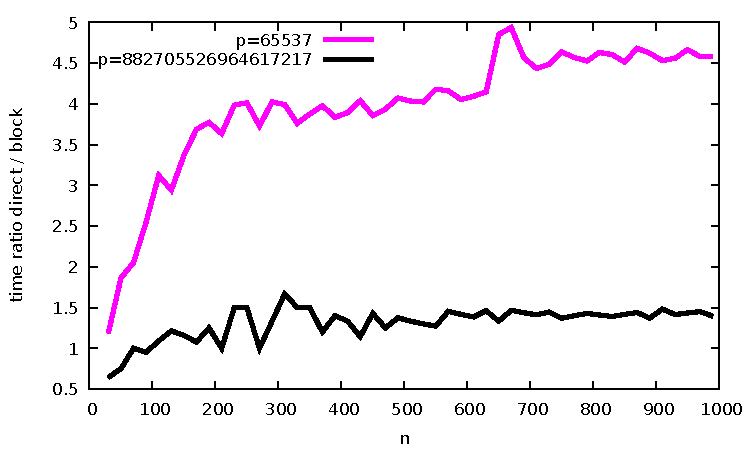
\includegraphics[width=7cm]{ratio-block-eschost-desktop.pdf}

We consider next the divide-and-conquer algorithm. The key factor for
the efficiency of this algorithm is the cost of multiplying an $n
\times n$ Cauchy-like matrix of displacement rank $\alpha$ by $\alpha$
vectors. We compare the approach of cost $O(\alpha^2 \M(n))$ of
Remark~\ref{rmk:factor3} to the algorithm of~\cite{BoJeMoSc16}, with
cost $O(\alpha^{\omega-1} \M(n))$, with a view of determining for what
values of $\alpha$ (if any) the latter becomes useful.

For the former algorithm, because we are able to cache several FFTs,
we found it slightly more advantageous to use NTL's FFT rather than
TFTs. The runtime of the first algorithm then displays the typical FFT
staircase behavior, so that as $n$ grows, the crossover value for $\alpha$
fluctuates, roughly between $30$ and $55$. The following graph shows
the time ratio between the algorithm of~\cite{BoJeMoSc16} and the
direct one, for $\alpha=60$; at best, the new algorithm wins by a
factor of 2. The results do not depend much on the nature of the prime
(since polynomial arithmetic is a significant part of the runtime, and
behaves essentially in the same manner, independently of $p$).

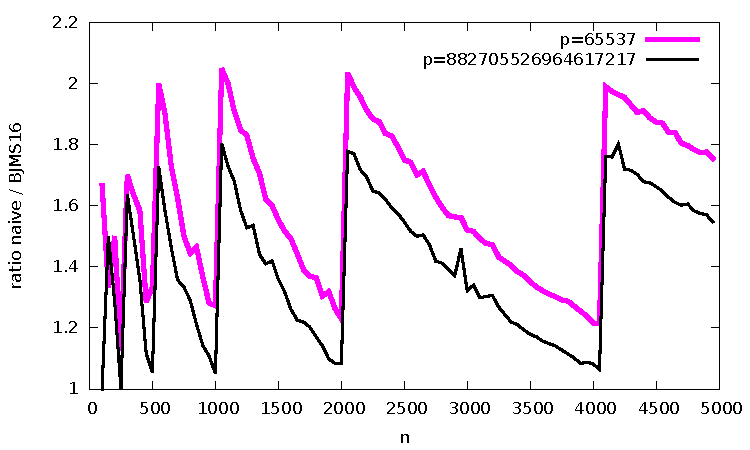
\includegraphics[width=7cm,height=4.1cm]{ratio-mul-matrix-eschost-desktop.pdf}

Using these results, we determined empirical crossover values
$\nu_0(\alpha)$ to end the recursion in the divide-and-conquer
algorithm and switch to the iterative algorithm. We expect
$\nu_0(\alpha)$ to grow with $\alpha$, since it
behaves like the solution of $\alpha n^2 = \alpha^2 \M(n) \log(n)$
(assuming here we do not use fast linear algebra, for simplicity). The
following table reports some values for $\nu_0$ (obtained by searching
for $\nu_0$ in increments of $100$).  The threshold is higher for
small primes, since such primes benefit more from our new iterative
algorithm.

\vspace{1mm}

\centerline{
{\small
\begin{tabular}{|c||c|c|c|c|c|c|c|}\hline
  $\alpha$ & 1 & 5 & 10 & 15 & 20 & 25 &30 \\\hline\hline
$p=65537$  & 400 &400 &500  &1000  &2000  &3300  &4200 \\\hline
$p\simeq 2^{59}$  & 200 & 400 & 400 & 700 & 1300 & 1600 & 2000\\\hline
\end{tabular}
}
}

\vspace{1mm}


These values being set, we show runtimes for solving
Problem~\ref{pb:cauchy} modulo $p=65537$ and
$p=8827055\-26964617217$, for increasing values of $n$, with
$\alpha=5$ and $\alpha=50$; we also show the runtime of a dense
matrix inversion in the same size. For a small displacement rank
such as $\alpha=5$, the runtime is essentially the same for these two
primes; with $\alpha=50$, we observe a difference, by a factor of up to 3. In any case, there is a clear gain
over dense methods.

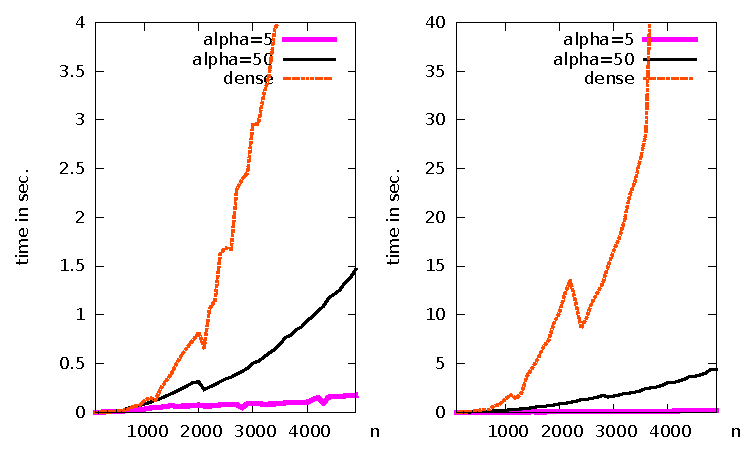
\includegraphics[width=8cm,height=4.4cm]{large_n-eschost-desktop.pdf}

We also determined, for a given value of $n$, the crossover value
$\alpha_0$ above which dense linear algebra becomes faster than
structured methods.  The value $\alpha_0(n)$ grows quite regularly
with $n$, good approximations being $\alpha_0(n) \simeq 0.2 n$ (for $p
< 2^{23}$) and $\alpha_0(n) \simeq 0.25 n$ (for larger values of
$p$). This means that there is a wide range of inputs for which
structured methods can be of use.

Our solution of Problem~\ref{pb:mosaic} is a direct reduction to the
Cauchy-like case. Putting the problem into Cauchy form by means of the
formulae of Eq.~(\ref{eq:gentoetogencau}) accounts for a small
fraction of the total runtime: between 5\% and 10\% for small $\alpha$
(say $\alpha < 10$), and less than 5\% for larger values of $\alpha$,
in all instances we considered.  

In the thousands of experiments we made, for matrix
sizes such as $n \ge 5000$ and small primes such as $p=65537$, we
observed some instances where the Cauchy matrix did not have generic
rank profile. This never happened for $p$ having more than $50$ bits.

%%%%%%%%%%%%%%%%%%%%%%%%%%%%%%%%%%%%%%%%%%%%%%%%%%%%%%%%%%%%
%%%%%%%%%%%%%%%%%%%%%%%%%%%%%%%%%%%%%%%%%%%%%%%%%%%%%%%%%%%%
%%%%%%%%%%%%%%%%%%%%%%%%%%%%%%%%%%%%%%%%%%%%%%%%%%%%%%%%%%%%

\vspace{-5px}
\section{Modular techniques}\label{sec:lifting}

We now address Problem~\ref{pb:mosaic} in the particular case where
$\K=\Q$. Several {\em modular algorithms} are available to solve dense
linear systems over $\Q$. A first option relies on the Chinese
Remainder Theorem, solving the system modulo several primes
$p_1,p_2,\dots$ before reconstructing the solution, making sure to
ensure consistency of the modular solutions when ${\rm ker}(\mT)$ has
dimension more than $1$. Other approaches such as Dixon's
algorithm~\cite{Dixon82}, Newton iteration or divide-and-conquer
algorithms use one prime $p$, and lift the solution modulo powers of
$p$.

Newton iteration for structured matrices goes back to Pan's
article~\cite{Pan92} (for Toeplitz-like matrices), and is explained in
detail in~\cite[Chapter~7]{Pan01}. To the best of our knowledge, the
other approaches mentioned above have not been discussed in the
literature on structured matrices, save for the second author's PhD
thesis~\cite{Lebreton12}. Our goal in this section is to first
briefly present some of these techniques and analyze their complexity
for the problem at hand; we will then discuss their practical
performance. We will highlight in particular the case of algebraic
approximants, for which we are able to obtain significant
improvements.

We denote by $\mathscr{I}:\mathbb{N} \to \mathbb{R}$ a function such
that integers of bit size at most $d$ can be multiplied in
$\mathscr{I}(d)$ bit operations; we can take $\mathscr{I}(d)=O(d
\log(d) \log\log(d))$ or $\mathscr{I}(d)=d \log(d)
2^{O(\log^*(d))}$~\cite{ScSt71,Furer07}. As in~\cite{GaGe13}, we
assume that $d\mapsto \mathscr{I}(d)/d$ is non-decreasing.

%%%%%%%%%%%%%%%%%%%%%%%%%%%%%%%%%%%%%%%%%%%%%%%%%%%%%%%%%%%%

\vspace{-5px}
\subsection{Solving square systems by lifting}
\label{ssec:liftsquare}

In this subsection, we are given a prime power $p^t$, where $t$ is a
power of 2, an $n \times n$ matrix $\mA$ and a vector $\vb$, both with
entries modulo $p^t$, and we assume that $\mA$ is invertible modulo
$p^t$, with inverse $\mB$. We discuss algorithms that solve the
equation $\mA \vx = \vb$, and we estimate their complexity when $\mA$
is a structured matrix. To simplify the cost analysis, we assume here
that $p=O(1)$.

We take $\CA$ such that, for any $t$, we can compute $\mA \vx \bmod
p^t$ in $O(\CA \I(t))$ bit operations, given a vector $\vx$ with
entries defined modulo $p^t$. Below, we will assume that $\mA$ is
Cauchy-like as in Remark~\ref{rmk:factor3}, and given by generators of
length $\alpha$, so that we can take $\CA \in O(\alpha \M(n))$. We
will see however that in the case of algebraic approximants, better
estimates are available.

We consider two approaches: a divide-and-conquer algorithm and Newton
iteration, which both feature a running time linear in the target
precision $t$.  We start with the divide-and-conquer approach. A
version of it is in~\cite{BeLe12} for dense matrices; the PhD
thesis~\cite{Lebreton12} describes this algorithm for Toeplitz-like
matrices.

% \vspace{-1mm}
\begin{algorithm}[h]
\setstretch{0.1}
  \LinesNumbered \DontPrintSemicolon
  \caption{Divide-And-Conquer algorithm $\DACQ$ \label{algo:dacQ}}

  \Input{$\mA$, $\vb$, $\mB \bmod p$, $p$, $t$ as above}
  \Output{a solution of  $\mA \vx = \vb$ mod $p^t$}

\lIf{$t = 1$}{\Return $\mB \, \vb$ mod $p$}

Compute $\vx_0 = $\DACQ($\mA$, $\vb$, $\mB$, $p$, $t/2$)\;

Compute $\vr_0 = \left( \mA \vx_0 - \vb\right) \bmod p^t$ and
$\vr_1 = r_0/ p^{t/2}$\;

Compute $\vx_1 = $\DACQ($\mA$, $\vr_1$, $\mB$, $p$, $t/2$)\;

\Return $\vx_0 - p^{t/2}  \vx_1$ mod $p^t$
\end{algorithm}
% \vspace{-2mm}

Assume that we have obtained generators of length $\alpha$ for $\mB$,
for instance by applying the algorithm of the previous section.  Thus,
at the leaves of the recursion, each product $\mB \vb$ mod $p$ can be
computed using $O(\alpha \M(n))$ bit operations; using our assumption
on $\I$, the total runtime is then $O(\CA \I(t) \log(t) +\alpha \M(n)
t)$ bit operations. With our upper bounds on $\CA$, this simplifies
further as $O(\alpha \M(n) \I(t) \log(t))$.

We turn next to Newton iteration. The matrix form of Newton iteration
computes the inverses $\mB_k=\mA^{-1} \bmod p^{2^k}$ by $\mB_{k+1} =
2\mB_k - \mB_k \mA \mB_k \bmod p^{2^{k+1}}$; once they are known, we
deduce the solution to our system by means of a matrix-vector product.

Let $(\mG,\mH)$ be generators for $\mA$. Pan's insight was to use the
relation above to compute the generators $(\mX,\mY)=(-\mB
\mG,\mB^{t}\mH)$ for $\mB$. Given $(\mX_k,\mY_k)=(\mX,\mY) \bmod
p^{2^k}$, we can reconstruct $\mB_k$, but to deduce
$(\mX_{k+1},\mY_{k+1})$, we have to multiply $\mG$ and $\mH$ by
$\mB_{k+1}$ or $\mB_{k+1}^t$. This is done using the expression for
$\mB_{k+1}$ above, which gives
\begin{align*}
\mX_{k+1} &= -(2\mB_k - \mB_k \mA \mB_k)\phantom{^t\,} \mG \bmod p^{2^{k+1}}\\
\mY_{k+1} &= \phantom{-}(2\mB_k - \mB_k \mA \mB_k)^t\, \mH \bmod p^{2^{k+1}}.
\end{align*}
This time, we are multiplying $\mA$ and $\mB_k$ (and their transposes)
by matrices of size $n \times \alpha$, all computations being done
modulo $p^{2^{k+1}}$. Each multiplication by {\em one} vector takes
$O(\alpha \M(n) \I(2^k))$ operations (even if $\CA$ is less
than $O(\alpha \M(n))$, multiplications by $\mB_k$ are the
bottleneck). Since we  multiply these matrices by $\alpha$
vectors, taking all steps into account, we arrive at a total of
$O(\alpha^2 \M(n) \I(t))$ bit operations. Using the algorithm
of~\cite{BoJeMoSc16}, this can be further reduced to
$O(\alpha^{\omega-1} \M(n) \I(t))$; this improvement was not
implemented.

Altogether, because it computes (generators of) a whole inverse,
Newton iteration is slower by a factor $\alpha$ (or slightly less, if
we use~\cite{BoJeMoSc16}); on the other hand, it saves a factor of
$\log(t)$. This is similar to what one observed when comparing these
techniques for e.g. the solution of differential
equations~\cite{BoChOlSaScSc07,BoChLeSaSc12}.

%%%%%%%%%%%%%%%%%%%%%%%%%%%%%%%%%%%%%%%%%%%%%%%%%%%%%%%%%%%%

\vspace{-5px}
\subsection{Solving Problem~\ref{pb:mosaic}}\label{ssec:liftQ}

The techniques above allow us to solve instances of
Problem~\ref{pb:mosaic}, that is, find nullspace elements for a
mosaic Toeplitz matrix $\mT$, but they would require the knowledge of
a maximal invertible minor of it. However, there is no guarantee that
$\mT$ possesses such a minor that would be mosaic Toeplitz as well,
and we do not know how to find it efficiently. Hence, we rely on the
transformation to the Cauchy structure / regularization technique
of Section~\ref{sec:basics}.

Over $\Q$, this approach has a certain shortcoming: the output is a
vector
%
%$\vb=\mW_{\vv}[(-\mA_r^{-1}\vc)^t ~ \vc^t]^t$
$\vb=\mW_{\vv}
\left[\begin{smallmatrix} 
-\mA^{(r)}_{0,0}{}^{-1} \mA^{(r)}_{0,1} \vc \\ 
\vc
\end{smallmatrix}\right]$
%
, with $\mA=\mV_\vu \mT \mW_{\vv}$, $\mA^{(r)}_{0,0}$ a maximal minor
of it and $\vc$ a random vector in $\K^{n-r}$, and due to the
preconditioning, the entries of $\vb$ are expected to be of large
height (larger than what we may expect for a solution of $\mT$). When
${\rm ker}(\mT)$ has dimension $1$, we are not affected by this
issue. Indeed, in this case, all solutions are of the form
$\lambda \vb_0$, for some vector $\vb_0 \in \Z^n$ whose bit-size can
be bounded only in terms of $\mT$. Hence, it suffices to compute the
solution $\vb$ of the regularized system modulo a large enough integer
$N$ and normalize it by setting one of its entries to $1$; this gives
us the normalization of $\vb_0 \bmod N$.

This idea could be extended to the case of an arbitrary nullspace
dimension, but it would be tantamount to lifting a whole nullspace
basis. Instead, we will reduce the nullspace dimension by adding a new
block of equations; when ${\rm ker}(\mT)$ has moderate dimension, this
barely affects the overall runtime (for particular applications to
algebraic approximants, another solution is described below).

For simplicity, we discuss here a version of the algorithm that may
run forever in unlucky cases. We choose a prime $p$ and compute
$\nabla_{\vu,\vv}$-generators for $\mA = \mV_\vu \mT \mW_{\vv}$ (mod
$p$), for $\vu,\vv$ as in Remark~\ref{rmk:factor3}. We call the
algorithm of the previous section, in order to determine the rank of
$\mA$; if $\mA$ does not have generic rank profile, choose another
$\vu,\vv$. After an expected $O(1)$ attempts, we obtain the rank of
$\mA$ (as a matrix over $\mathbb{F}_p$), and thus the dimension $s$ of
its nullspace. If $s$ is greater than one, we add a block of Toeplitz
matrices having $s-1$ rows to $\mT$, with small random entries, and
update $\mA$ accordingly. Heuristically the new matrix $\mT$ has
nullspace dimension $1$ (otherwise, add another block of equations).

Let $d={\rm rank}(\mT)$, $\mA_{d}$ be the $d \times d$ top-left
submatrix of $\mA$, and $\vb_d$ be the vector of the first $d$ entries
of the last column of $\mA$. We assume that $\mA$ has generic rank
profile, so that $\mA_{d}$ is invertible.  We compute
$\vx = \mA_d^{-1} \vb_d$ (mod $p$) and
$\vy = \mW_\vv [x_1, \cdots, x_d, -1]^t$ (mod $p$), we normalize $\vy$
by dividing it by its first non-zero entry, and we set $t=1$.  While
we either cannot apply rational reconstruction to the entries of
$\vy$, or after applying rational reconstruction to $\vy$ we have
$\mT \vy \ne 0$, we do the following: set $t = 2t$, update modulo
$p^t$ the quantities $\mA_{d}$, $\vb_d$, $\vx$ (use one of the
algorithms of Section~\ref{ssec:liftsquare}) and $\vy$, and divide
$\vy$ by its first non-zero entry.

% \begin{enumerate}
% \item set $t = 2t$ and update $\mA_{d}$ and $\vb_d$ (mod $p^t$);
% \item compute $\vr = \mA_d \vx - \vb_d$ (mod $p^t$) and
%   $\vr_1 = \vr / p^{t/2}$;
% \item call one of the algorithms in the previous subsection to find
%   $\vx'$ such that $\mA_d \vx' = \vr_1$ (mod $p^{t/2}$);
% \item set $\vx = \vx - p^{t/2} \vx'$,
%   $\vy = \mW_\vv [x_1,\cdots,x_d,-1]^t$ (mod $p^{t}$), and divide
%   $\vy$ by its first non-zero entry.
% \end{enumerate}

A complete analysis of this algorithm would quantify the primes of bad
reduction, give bounds that allow us to stop lifting the solutions if
we reduced modulo such a bad prime and study the previous reduction to
nullity one of $\mT$; we leave this to future work.  In any case, if
the lifting stops, we have obtained a solution to our system. Due to
the doubling nature of this procedure, the runtime is proportional to
that of the algorithm for solving square systems used at line 3, plus
the cost of rational reconstruction. The former is
$O(\CA \I(t) \log(t) +\alpha \M(n) t)$ bit operations using
divide-and-conquer, and $O(\alpha^2 \M(n) \I(t))$ or
$O(\alpha^{\omega-1} \M(n) \I(t))$ using Newton iteration; the latter
is $O(n \I(t) \log(t))$.

Finally, we mention the cost of Chinese Remaindering techniques:
instead of computing the solution modulo the $t$-th power of a single
prime $p$, we might want to solve the system modulo $t$ primes of the
same magnitude.  If we assume that $\mA$ remains invertible with
generic rank profile modulo all these primes, and all these primes are
$O(1)$, the runtime for solving the systems is now $O(\alpha^{2} \M(n)
\log(n) t)$ or $O(\alpha^{\omega-1} \M(n) \log(n) t)$, by the results
of Section~\ref{sec:abstract} (to this, we have to add the cost $O(n
\I(t) \log(t))$ of Chinese Remaindering and rational reconstruction).


We conclude this subsection with an important
particular case, the computation of algebraic approximants. We are
given a power series $f$ in $\Q[[x]]$, together with degree bounds
$d,e$; our goal is to compute a polynomial $P \in \Q[x,y]$, with
$\deg(P,x) \le d$, $\deg(P,y) \le e$, such that $P(x,f) = 0$.
For any $\sigma \ge 0$, finding $P$ with the above degree bounds and
such that $P(x,f) = 0 \bmod x^\sigma$ is a Hermite-Pad\'e
approximation problem of a very special kind (all input series are
powers of $f$). To our knowledge, no algorithm in the framework of
Section~\ref{sec:abstract} can exploit this extra structure;
in the case of computations over $\Q$, we will now see that
improvements are possible.

First, we show how to simplify the reduction to nullity one.
Th\'eo\-r\`eme~7.15 in~\cite{BoChGiLeLeSaSc17} shows that if such a
$P$ exists and is irreducible, then any $Q \in \Q[x,y]$ with the same
degree bounds as above and such that $Q(x,f) = 0 \bmod x^{2de+1}$ is a
multiple of $P$.  From this, one deduces easily that if we compute
\emph{two} such polynomials $Q_1,Q_2$, their GCD will generically be
$P$ itself. For all primes $p$ except a finite number, the rank of our
matrix $\mT$ does not change modulo $p$, and the GCD of two random
basis elements commutes with reduction modulo $p$ (note that $P \bmod
p$ may not be irreducible anymore). Hence, we can (probabilistically)
find $P \bmod p$ by computing two solutions $Q_1,Q_2$ to the above
Hermite-Pad\'e problem modulo $p$ and taking their GCD. This reveals
the support of $P$; we can then refine the degree bounds in our
Hermite-Pad\'e problem, which in turn reduces the nullity of matrix
$\mT$ to $1$.

Next, we show how to speed-up algorithm $\DACQ$ in this case. The
block-Toeplitz matrix $\mT$ of our Hermite-Pad\'e problem has
displacement rank $\alpha = O(e)$, with $e+1$ Sylvester blocks having
$O(d)$ columns and $O(de)$ rows; as a result, the naive estimate on
the cost of the matrix-vector product by matrix $\mA = \mV_\vu \mT
\mW_\vv$ is $\CA=O(e \M(de))$. However, we can reduce this cost using
baby-steps / giant steps techniques: the bivariate modular composition
algorithm of~\cite{NuZi04} shows that we can do matrix-vector product
by $\mT$ using $O(e^{1/2} \M(de) + e^{(\omega+1)/2} \M(d))$
operations; since multiplications by $\mV_\vu$ and $\mW_\vv$ take
$O(\M(de))$, we obtain the improved estimate $\CA=O(e^{1/2} \M(de) +
e^{(\omega+1)/2} \M(d))$ in this case. Algorithm $\DACQ$ is the only
algorithm we know of that takes into account the extra structure of
algebraic approximants; we expect that similar improvements are
possible for {\em differential approximants}, using the evaluation
algorithm of~\cite{BoSc09}.

\vspace{-5px}
\subsection{Experimental Results}

Our experiments are dedicated to solving instances of Hermite-Pad\'e
approximation, which is a useful particular case of
Problem~\ref{pb:mosaic}. We discuss two families of problems, first
the approximation of general power series, then algebraic
approximants. Timings are measured on the same machine as
Subsection~\ref{ssec:exp1}.

In both cases, we show two graphs: on the left, we have five blocks,
each with $n$ columns; on the right, we have $n$ blocks, each with $n$
columns.  With the notation of the introduction, this means we are
looking for approximants $(p_0,\dots,p_4)$, resp.\
$(p_0,\dots,p_{n-1})$, with degree bounds $(n,n,n,n,n)$, resp.\
$(n,\dots,n)$. The displacement rank $\alpha$ of these matrices if
$6$, resp.\ $n+1$.

We first examine the results for general power series. Our experiments
showed that the runtime grows predictably with respect to the input
bit-size; as a result, we fix the input coefficients to be 10 bit
integers, so the number of lifting steps depends just on~$n$.

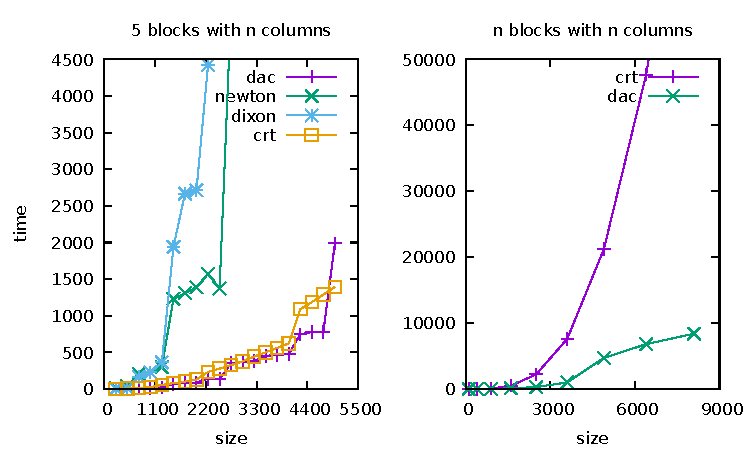
\includegraphics[width=7cm]{plots/compare-general.pdf}

Matrices are generated so as to have $1$ less row than they have
columns; since the inputs are random, they have nullspace of dimension
$1$ (we also generated instances with nullity up to 10; using our
heuristic to reduce nullity, runtimes were almost
indistinguishable). The primes we use have 59 to 60 bits.  For $\DACQ$
and Newton iteration, the sharp increases indicate an additional
lifting step.

Newton iteration is slower than $\DACQ$, especially when the number of
block grows (since its runtime is quadratic in the displacement rank
$\alpha$). Newton iteration should theoretically be competitive with
$\DACQ$ when the number of blocks is fixed, and the size (and thus the
output bit size) grow, since its theoretical runtime is better by a
$\log(t)$ factor, where $t$ is essentially the output bit
size. However, this is not noticeable on our experiments: in practice,
the integer multiplication function $\I(d)$ grows like
$d^{1+\varepsilon}$, for some $\varepsilon > 0$; in that case, the
analysis of $\DACQ$ can be refined to $O(\alpha \M(n) \I(t))$. 

CRT, on the other hand, seems to be competitive with $\DACQ$ when
$\alpha$ is small but is significantly worse as $\alpha$ grows: the
runtime CRT is not linear in $\alpha$, while $\DACQ$ is. 

Next, we examine the computation of algebraic approximants; on the
basis of the previous experiments, we consider algorithm $\DACQ$ only.
We start by generating a bivariate polynomial $P(x,y)$ and compute one
of its power series solutions $f$. Since we expect the coefficients of
$P$ to be smaller than the coefficients of $f$, we can better control
the behavior of the algorithms by choosing the bit size of $P$ (here,
it was fixed to be 1000 bit integers).  We compare algorithm $\DACQ$
as in the general case, with $\CA=O(\alpha \M(n))$, to the improved
version using the bivariate modular composition (BMC) algorithm
of~\cite{NuZi04} described above, featuring a lower value for
$\CA$. The latter algorithm uses polynomial matrix multiplication,
which we implemented using reduction modulo FFT primes and TFT
polynomial multiplication.

As a result, we can see a significant difference between the two
algorithms as the size of the matrix grows: the theoretical speed-up
predicted in Subsection~\ref{ssec:liftQ} is observed in practice.

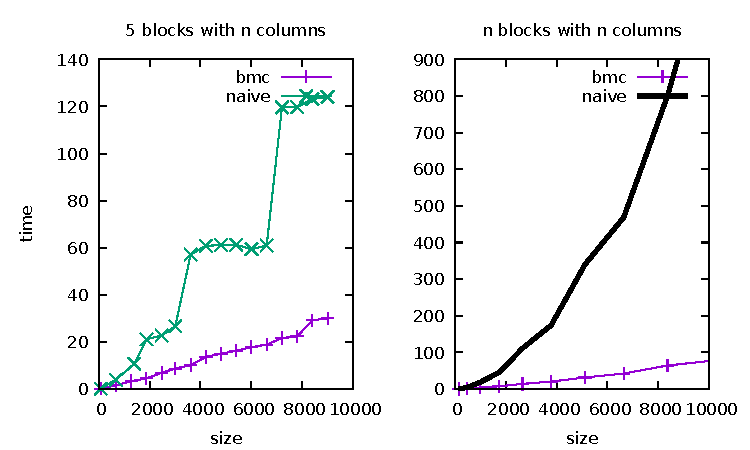
\includegraphics[width=7cm]{plots/compare-algebraic.pdf}

Overall, the divide-and-conquer lifting algorithm turned out to be the
most efficient method in all our experiments, especially as it can
take extra structure into account, as in the case of algebraic
approximants.



\bibliographystyle{plain} {\tiny \bibliography{structured}}


\end{document}
